\title{\textbf{Automatic Projector Tilt Compensation System}}
\author{Ganesh Ajjanagadde \quad Shantanu Jain \quad James Thomas}
\date{\today}
\documentclass{article}

\usepackage{amsmath} % for math
\usepackage{graphicx} % for including images
\usepackage{float} % for floating figures, i.e can place/modify images in fancy ways
\usepackage{verbatim} % for block comments in the source file
\usepackage{hyperref} % for useful hyperlinks over the document
\usepackage{natbib} % for bibliography
\usepackage{minted} % for source code listing
% NOTE: MINTED HAS SOME INSTALLATION/USAGE INSTRUCTIONS, SINCE IT ``SHELLS-OUT'' TO PYTHON
% SEE DOC AT https://github.com/gpoore/minted
%\usepackage[margin=1in]{geometry} % for adjusting margins

%Please place images in img/ subdir of proj_report for clean directory structure

\begin{document}
\maketitle

\begin{abstract}
We designed a system that corrects the input to a projector if it is tilted so that its output appears unskewed.
We read input from a NTSC (National Television System Committee) video camera and store it in an internal block memory.
We then process the frame stored in memory using a perspective transformation to pre-warp the image that is sent to the projector via a VGA (Video Graphics Array) signal.
The parameters of the perspective transformation are obtained from an accelerometer, which senses two axes of tilt.
This allows automatic keystone correction in the two directions sensed by the accelerometer provided the output screen is vertical.
Our method also includes options for manual keystone correction to any degree desired, for any projector and screen orientations.
For ease of manual correction, we provide the option of using a test pattern (a checkerboard).
We also play some useful audio for the percentage of pixels kept by the transformation.
\end{abstract}

\newpage
\section*{Acknowledgments}
First and foremost, we would like to thank our 6.111 instructor Gim Hom for his tremondous patience, experience, and intuition regarding digital systems.
This project would never have been possible without him,
and countless number of times he saved our group a huge amount of time by some very critical observations.
Not only that, he also played a very important role in our choice of project topic.
Initially, we were planning to create some sort of Bitcoin miner.
I think it is safe to say that we are all glad that we chose this topic instead on his suggestion.

We would also like to thank all the teaching assistants, lab assistants, and CI-M writing instructors for their very useful suggestions and feedback.
We particularly appreciate the guidance of one of our TA's Jos\'{e} E. Cruz Serall\'{e}s for his wealth of experience with Verilog and Xilinx's tools.
His project on recursive augmented reality was also very useful as a reference point for certain aspects,
such as generation of clocks of different frequencies and the correct timing of sync and blank signals for a $640 \times 480$  @60 Hz VGA display.
Furthermore, he was able to identify a subtle bug with our memory address computation.

Last, but not least, we would like to thank all our peers in this class.
Their thoughtful questions during our proposal presentation raised issues that we had not anticipated.
Furthermore, they often were willing to help with some commonly faced issues in the lab, thereby avoiding duplication of effort.
We particularly appreciate the note on Piazza (our online discussion forum) by Andres Erbsen regarding test benches and use of Icarus Verilog.
\newpage

\tableofcontents
\newpage

\section{Introduction}
Due to the advances in semiconductor technology,
today's display projectors can incorporate fairly sophisticated digital processing algorithms for various enhancements to the visual appearance.
Moreover, there is an increasing prevalence of portable projectors that benefit from fast, automated setup.
One desired functionality is keystone/tilt correction.
In other words, even when the projector is tilted, the projector should be able to ``pre-warp'' the image so that its output appears unskewed.
\begin{center}
\begin{figure}[h!]
    \caption{Keystone Correction In Vertical Direction \url{https://en.wikipedia.org/wiki/File:Vertical-keystone.jpg}}
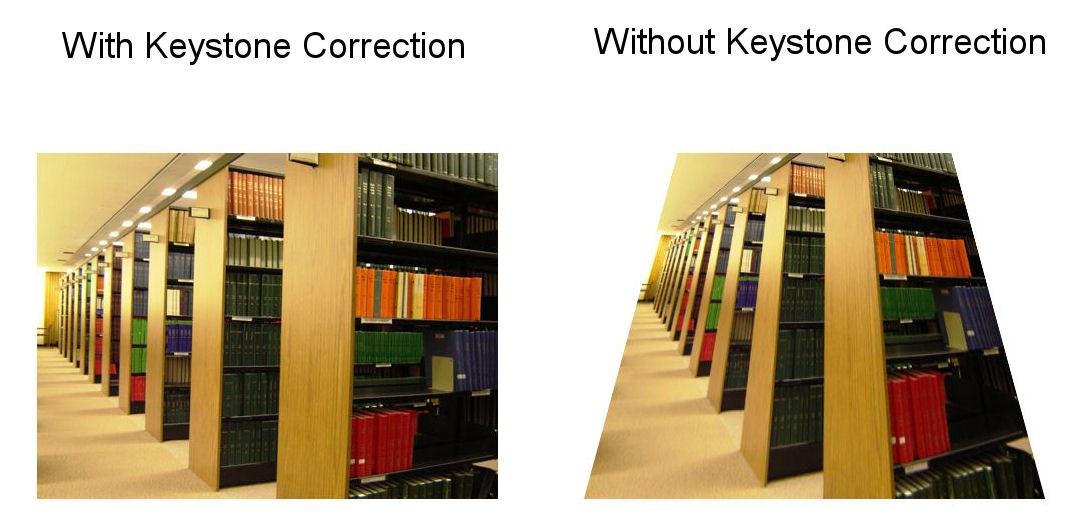
\includegraphics[width=0.8\textwidth]{./img/keystone}
\end{figure}
\end{center}

In this project, we project the output of a camera, connect the camera's output to the FPGA (Field Programmable Gate Array) board,
and the FPGA board's VGA output to the projector.
We mount an accelerometer on the projector and measure its signals to determine the projector's tilt angle on two axes.
We then run a perspective transformation algorithm on the FPGA that warps the camera output based on the tilt angles and produces the results at the VGA output for the projector to display.
We also provide a manual correction mode so that any desired correction can be achieved.
This manual correction mode is exposed to the user via the arrow keys and switches on the FPGA kit.
This is of use in mainly two cases:
\begin{itemize}
\item The automatic correction obtained using the accelerometer readings is unsatisfactory or inadequate.
\item The user desires to correct for projector orientation in the third axis, or in the case when the screen is non-vertical.
\end{itemize}
Finally, we also provide a useful voice output for the percentage of pixels kept after the perspective transformation (this is a lossy transformation in general).
The audio is triggered by pressing a button the FPGA kit.

% A comparison of the result without using our system versus using our system is provided below.
% TODO: ACTUAL IMAGE (I don't have these images)

\section{Previous Work}
Given the practical importance of keystone correction, there has been significant research on doing automatic keystone correction.
While \citet{raskar2001self} and \citet{sukthankar2001smarter} provide a solution to this problem, their methods suffer from one principal weakness,
already noted in \citet{baoxin2004automatic}, namely that their algorithms are not well suited for implementation in an embedded system.
For instance, their methods require solving an 8x8 system of linear equations via Gaussian elimination or similar methods,
which is not suitable for embedded platforms, particularly those with slow dividers.
Our key technical contribution is the elimination of the Gaussian elmination algorithm,
and instead replacing it with closed form solutions for the equations.
Moreover, we implement our algorithm on a 6 million gate Xilinx Virtex 2 FPGA, demonstrating that our algorithm is suitable for embedded systems use.
The work done in \citet{baoxin2004automatic} subsumes most of this work.
However, thier system is much more complex complex, as evidenced by the use of a camera for computing the precise perspective transformation.
For the scope of this term final project,
we use a simpler accelerometer based approach instead, paying the price of loss of automatic correction along one axis.
Note that we still retain fully general manual correction ability.

\section{Module Architecture}
Below is a block diagram including all of the major modules in our system, which are explained further below and in later sections:
\begin{center}
\begin{figure}[H]
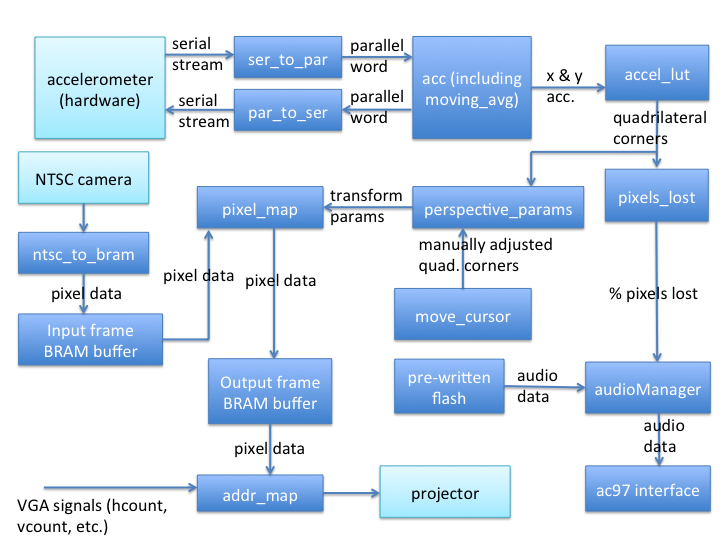
\includegraphics[width=\textwidth]{./img/block_diag}
\end{figure}
\end{center}

Our keystone correction system can be divided into roughly 4 sections:
\begin{enumerate}
\item Accelerometer interface
\item Perspective transformation
\item  I/O (Input/Output) interface
\item Audio system
\end{enumerate}

The accelerometer presents a SPI interface for data transfer. The par\_to\_ser module converts a multi-bit value to a serial stream of bits for transfer to the accelerometer. The ser\_to\_par module converts a serial stream of bits read from the accelerometer to a multi-bit value of desired width. The moving\_avg module computes the average of 32 accelerometer readings. The acc module uses the par\_to\_ser and ser\_to\_par modules to initialize the accelerometer and fetch x and y acceleration readings from it in a loop, averaging them using the moving\_avg module.

The perspective transformation section is where all core computations are computed.
The accel\_lut module accepts the accelerometer readings from the accelerometer as an index into a ROM (read-only memory) containing coordinates of four coordinates of a quadrilateral.
The corners of the quadrilateral (after multiplexing with manual override parameters) are fed into the perspective\_params module, which computes necessary perspective transformation parameters.
The perspective parameters are then fed into pixel\_map, which maps the screen rectangle onto the quadrilateral described above via a perspective transformation.
The pixels\_kept module is a side module that accepts the corners of the quadrilateral, and computes the percentage of pixels kept during the transformation.
This is of use in the audio system.

The input/output interface to various buttons/switches is contained in the top-level labkit.v file.
The relevant buttons/switches are passed to move\_cursor module, which manipulates the corners of the quadrilateral when the user wishes to manually adjust the correction.
The bram module implements a very simple 2 port block memory on the FPGA.
Two instances of this are created, one called ntsc\_buf storing the camera input, and one called vga\_buf containing the processed output (from the perspective transformation).
Essentially, we have a pipeline formed:
input camera writes to ntsc\_buf, perspective transformation reads from ntsc\_buf and writes to vga\_buf, and the output VGA signal is formed by looping over the vga\_buf.

TODO (SHAWN): BRIEF PARA ON AUDIO SYSTEM AT HIGH LEVEL

\section{Design Decisions}

There are a couple of noteworthy design decisions.

\subsection{Use of $640 \times 480$ @60 Hz VGA}
The first of them is the use of a $640 \times 480$ @60 Hz VGA display.
The use of $640 \times 480$  as opposed to the more common higher resolutions found today is due to the memory and computational limitations of our FPGA kit.
Initially, we hoped that we could get away with generic code that does not explicitly tie in heavily with the specific screen resolution.
Unfortunately, this is not easy, since the choice of resolution influences many different aspects.
Chief among these are the sizes of memory vs available memory tradeoff, the bit widths of $x$ and $y$ coordinates, the size of the accel\_lut ROM,
and the bit widths of numerous other quantites such as the dividers and the multipliers in pixel\_map and perspective\_params respectively.
The choice of 60 Hz was made on the basis of its almost guaranteed availability: almost all VGA displays support this refresh rate.

\subsection{Use of NTSC Camera as Input}
Also related to input/output is our decision to use an NTSC camera feed as the input to the FPGA.
Ideally, we would have liked to hook up a computer's VGA signal to the FPGA, so that we can demonstrate the correction system in a more realistic setting.
Unfortunately, the labkit in this course has only a single VGA port, ruling out this option.

\subsection{Choice of Memory Architecture}
The second major design decision made was the choice of memory architecture.
We initially planned on using the available 36 Mbits of ZBT memory spread across 2 banks.
This would allow us to store at least 4 frames at full $640 \times 480$  resolution and 24 bit color (8 bit R, 8 bit G, 8 bit B).
Unfortunately, it turns out that ZBT memory is not dual-ported, so read and write on the same bank can't be achieved simultaneously.
Since the perspective transform (operating pixel by pixel) turns out to be a huge computational bottleneck,
we did not want to waste additional time waiting for read/write on ZBT.
Moreover, coordination between the memory banks storing processed and unprocessed data would require some sort of arbiter, adding complexity to our project.
Thus, we chose instead to go with the block memory on the FPGA.
This can be made into true dual-port memory, and has a single read/write cycle latency, as opposed to the multi-cycle latency of ZBT memory.
However, the amount of block memory available on the FPGA is only 2.5 Mbits.
This required sacrifice on image quality.
We chose a combination of image downsampling and color depth reduction.
More specifically, we chose a 320x240 sized memory, with 12 bits per line (4 bit R, 4 bit G, 4 bit B).
This results in approximately 1 Mbit per buffer, and we use 2 buffers, leaving us with nearly 512k for the accel\_lut ROM.
That is more than sufficient for our accel\_lut.
It is certainly possible to squeeze some more color depth, e.g a 14 bit asymmetrical division among R, G, and B.
This should help the image quality, but our visual tests indicated no substantial improvement, and hence we omitted this.

\subsection{Choice of clocks}
The last noteworthy design decision is our choice of clocks.
To avoid clock domain issues, as much as possible we used multiples of a common system clock.
Using the Xilinx DCM (Digital Clock Manager), we synthesized a 50 MHz clock from the labkit's standard 27 MHz clock.
We used this as a global sys\_clk.
$640 \times 480$ @60Hz needs to be driven at nearly 25 MHz, and was thus obtained by multiplying the time period of sys\_clk by 2.
The NTSC camera must be driven at around 27 MHz, and the appropriate clock is already generated by the labkit.
To avoid change of the perspective parameters mid-frame, we also needed a slow\_clk signal,
i.e one who's time period is on the order of seconds.
This can't be accomplished through the use of DCM that easily.
Moreover, since actual timing violations for this signal are not really that important,
we implemented a simple ``flip clock on reaching a count'' style ``clock divider''.
TODO: SHAWN, ADD NOTE ON CLOCKS USED FOR AUDIO

\section{Module Descriptions}

In this section, we give a more detailed description of each module, along with the respective contributors.

\subsection{par\_to\_ser (James)}
This module converts a word of some size W (e.g. reg[W-1:0]) to a stream of bits, one at each clock cycle, to be sent to the accelerometer. The higher-order bits are produced first. This module is necessitated by the SPI communication protocol of the accelerometer.

\subsection{ser\_to\_par (James)}
This module converts a stream of bits received from the accelerometer, one per clock cycle, to a word of desired width. It expects that the higher-order bits will be received first.

\subsection{moving\_avg (James)}
This module uses a ring buffer to store the last 32 acceleration readings received from the accelerometer for a particular dimension. When a new sample is received, the oldest sample is removed, the sum of the last 32 samples is adjusted accordingly, and the average is recomputed. Since we compute the average over 32 ($2^5$) samples, we do not need dividers and can use bit shifts for the needed divisions. This module is meant to smooth acceleration readings, which are expected to fluctuate slightly even when the accelerometer is held fixed.

\subsection{acc (James)}
The timing diagram for 4-wire SPI interaction with the accelerometer is shown below:

\begin{center}
\begin{figure}[H]
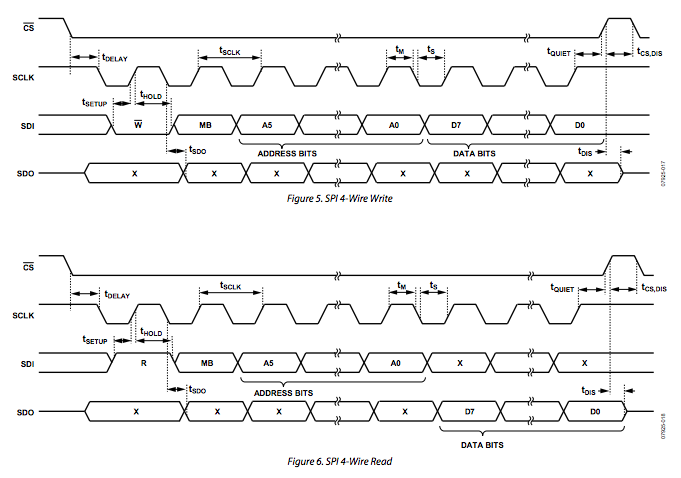
\includegraphics[width=\textwidth]{./img/acc_timing}
\end{figure}
\end{center}

This module first initializes the acclerometer and then reads x and y acceleration values from it in a loop. The clock used for accelerometer communications is our 50 MHz system clock slowed by a factor of 20, which meets the the max clock frequency spec of 5 MHz. Most of the default configurations for the accelerometer are acceptable for our purposes; the only initialization we need to do is set the measure bit of the POWER\_CTL register (each register contains a single byte). Since this register is at address 0x2D, and since we want to perform a single-byte write to it, we first drive the SDI pin with the serial bit stream 8'b00101101 (see Figure 5 in the timing diagram: upper two bits for mode and lower six bits for register address) to specify the mode and register address, and then drive it with the data to be stored in the register. By default, the accelerometer can measure acceleration values in the range of $\pm 2g$, which is sufficient for our purposes since we care only about static acceleration (which is in the range $\pm 1g$).

After 16 accelerometer clock cycles have passed, we know that we have sent all of the necessary initialization data to the accelerometer, and we transition our accelerometer state machine to the x-y read loop. Since the x and y acceleration readings are 16 bits (two registers' worth, since the accelerometer gives us 10 bits of precision), we want to perform a multi-byte read of the x and y registers, which can be done in the manner shown in Figure 6 of the timing diagram. We simply assert the R and MB bits, continue driving SDI with the address bits for the first x or first y register (the second registers for x and y immediately follow the first, which is why is multi-byte read of contiguous registers is acceptable), and then wait 16 additional cycles for all of our data to be produced on the SDO line. We rotate between a state for reading the x registers and a state for reading the y registers. We feed the produced x and y readings into instantiations of the moving\_avg filter, and the output of the acc module is the output of these filters.

One challenge we faced was getting the accelerometer clock period correct. Even though the spec states that the maximum clock frequency is 5 MHz, if we use a 5 MHz clock and then use a single clock cycle to implement the $t_{CS,DIS}$ waiting period shown in Figures 5 and 6 of the timing diagram, we will not meet the minimum $t_{CS,DIS}$ spec of 250ns. So we had to pick a clock frequency lower than 1s/250ns = 4 MHz to use a one-cycle wait to meet the $t_{CS,DIS}$ spec. This bug took quite a while to find.

Below is a picture of the accelerometer module working in isolation, with averaged accelerometer readings displayed on the hex display:
\begin{center}
\begin{figure}[H]
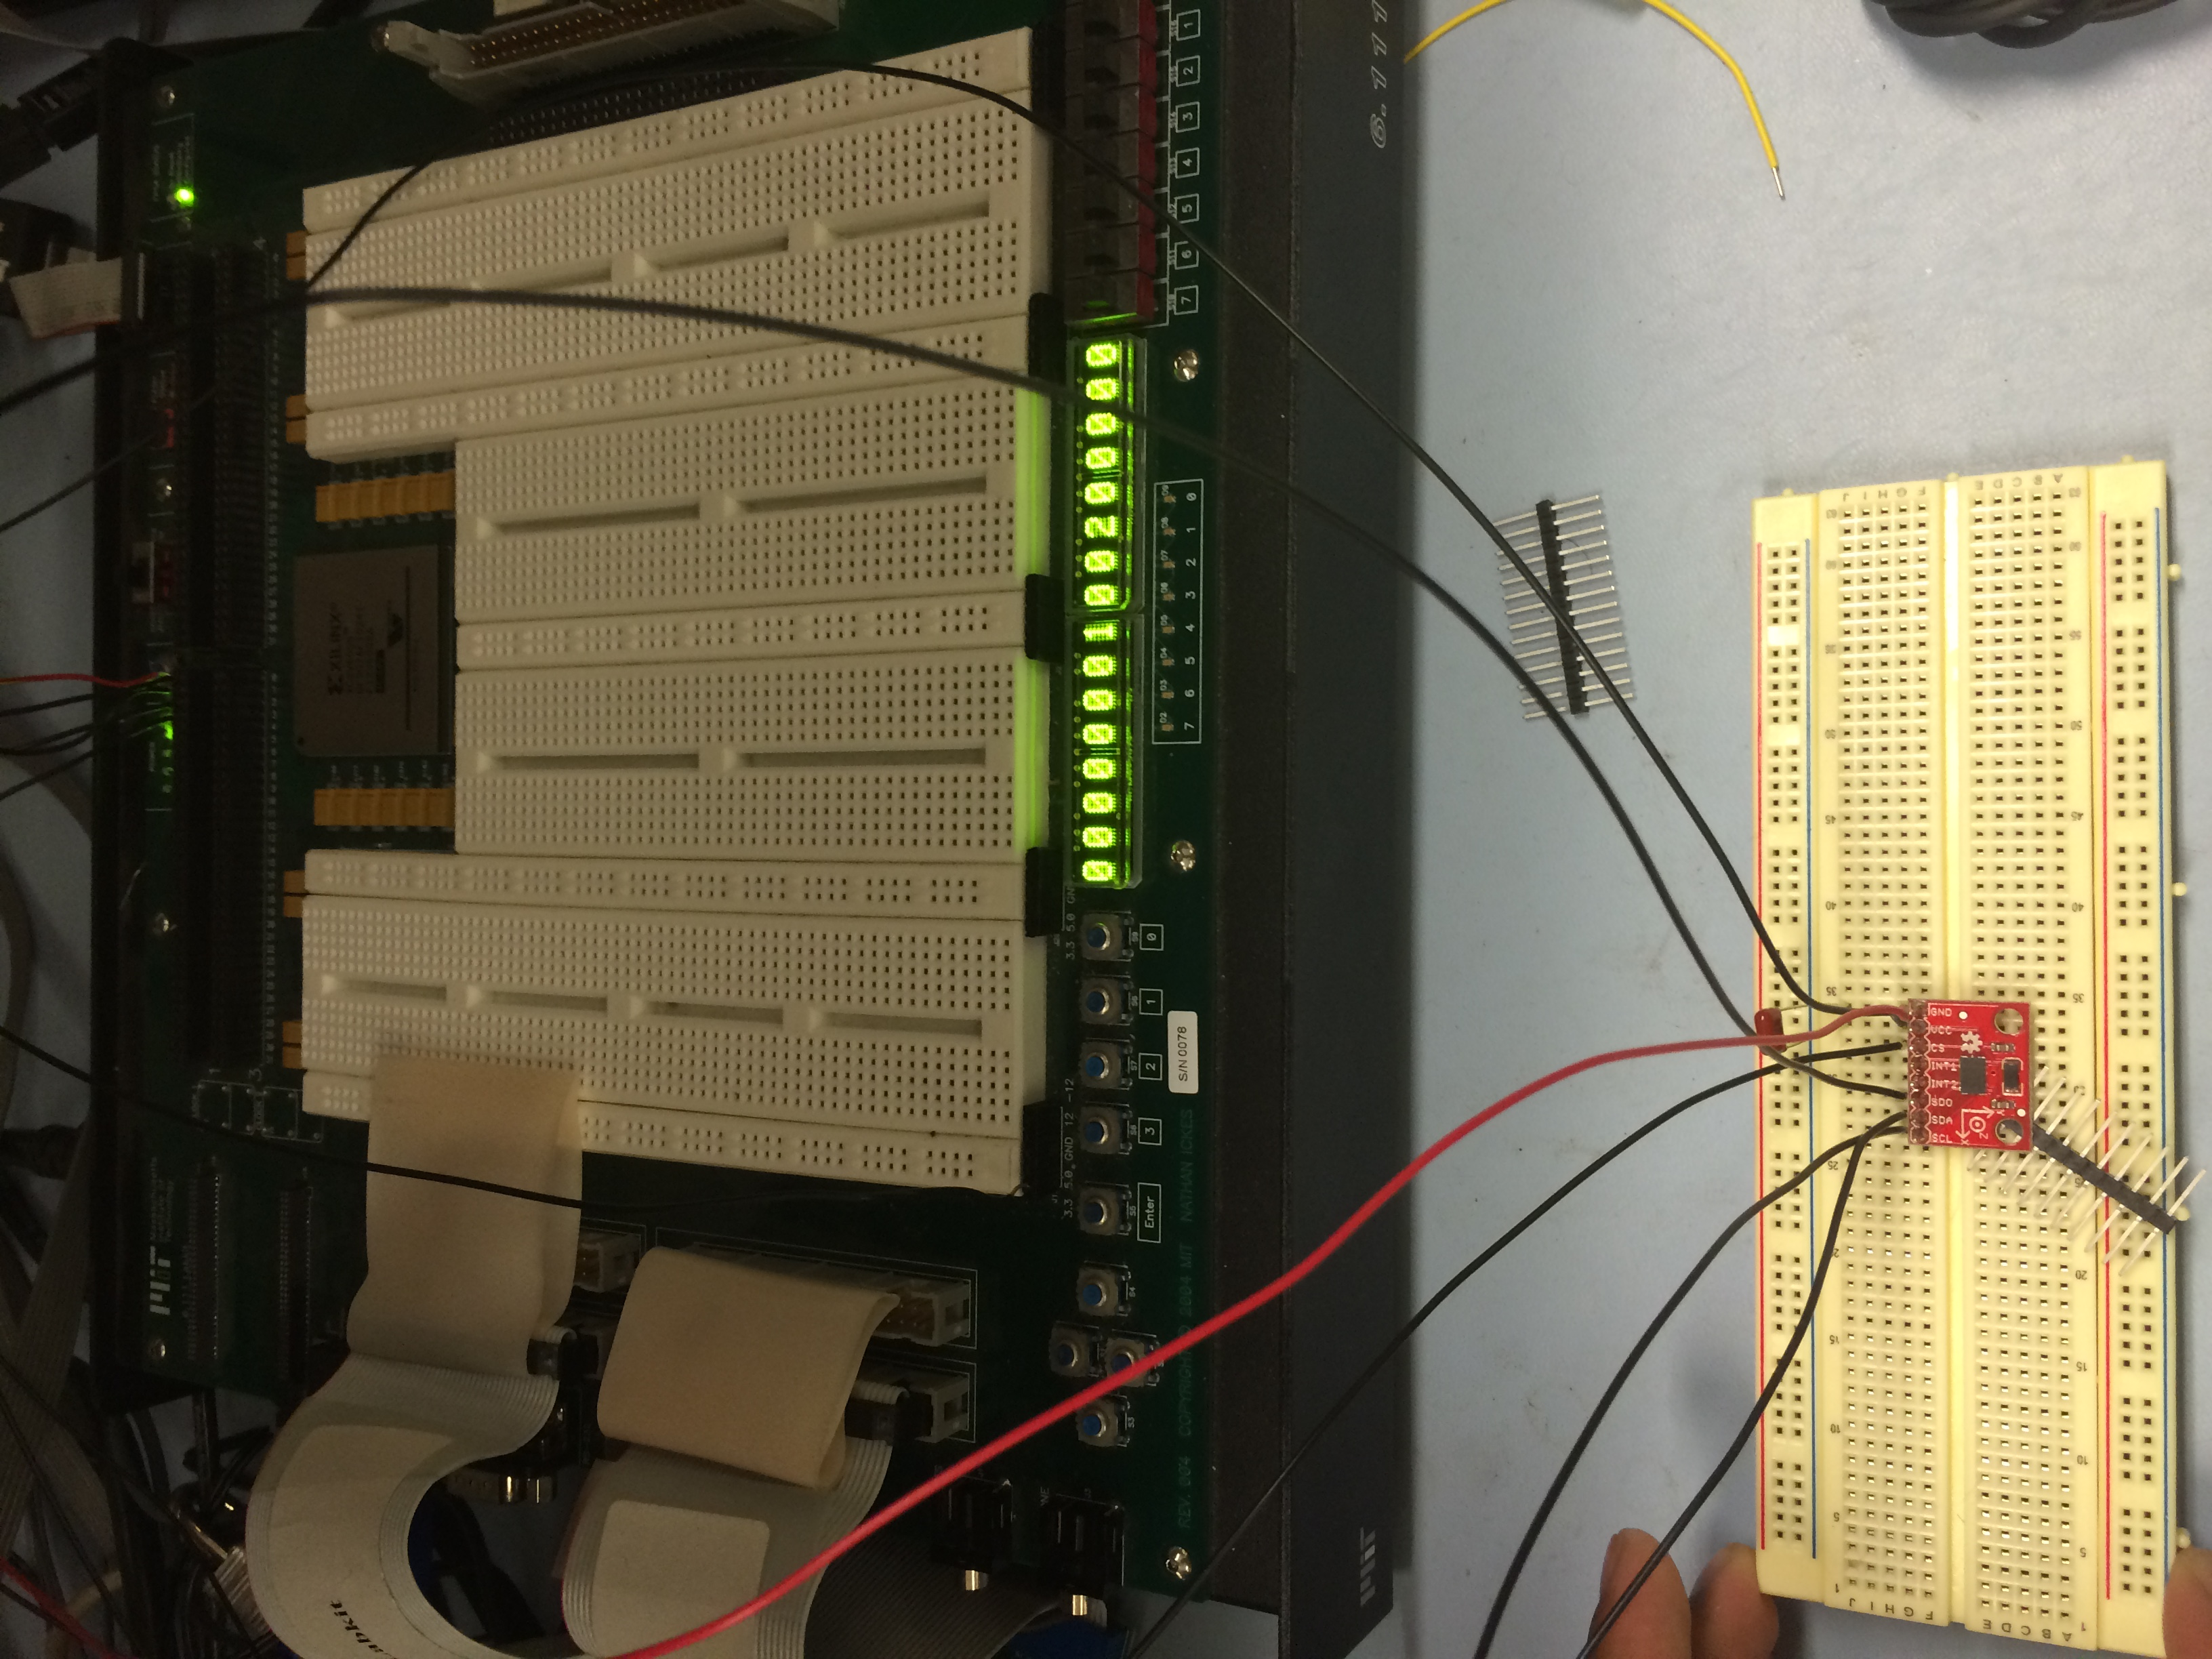
\includegraphics[width=0.8\textwidth, angle=270]{./img/accel-complete}
\end{figure}
\end{center}

\subsection{accel\_lut (Ganesh)}
The accel\_lut module provides a lookup table from the accelerometer readings in two directions to the four corners of the quadrilateral.
The output is synchronized to the global sys\_clk.
The module is essentially implemented as a giant case statement, from which Xilinx's tools are able to infer a ROM of the appropriate size.
Although the data coming out of the accelerometer has 10 bits of precision in each axis,
using the full precision would require too much space for the ROM.
Instead, we use 6 bits for each of the 2 axes, for a total of 12 bits as an index into the ROM.
Each word of the ROM is 76 bits wide.
This is because each $x$ coordinate is 10 bits wide (0 to 639), each $y$ coordinate is 9 bits wide (0 to 479), and there are 4 corners.
Since each entry corresponds to a choice of quadrilateral corners, and there are $2^{12} = 4096$ entries, manual entry of the lookup table is infeasible.
Instead, we wrote a code generator accel\_lut.jl in the Julia programming language (\url{julialang.org}).
Essentially, the code generator accepts an input CSV (comma separated values) file containing some entries of the desired lookup table obtained via manual testing.
The code generator then does a mathematical interpolation to obtain the remaining values of the lookup table, and writes out the accel\_lut.v file.
Of course, it may be argued that the interpolation is not sufficient to get fine grained accuracy.
Indeed, our demonstration did show that our lookup table could use some refinement.
However, we believe that this is not an inherent deficiency of the approach; it just means that we need more data points and sufficient polynomial degree of the interpolator.
Also related to this is another merit to this method: as the user obtains more and more entries,
he/she can simply populate the CSV file with them.
The quality of interpolation can then only improve.

\subsection{pixels\_kept (Ganesh)}
The pixels\_kept module accepts the four corners of the quadrilateral, computes its area, and expresses it as a percentage of the total area.
The area formula of a quadrilateral in terms of the coordinates of its four corners is a simple determinant expansion,
and may be found easily in elementary geometry references.
For a quadrilateral with coordinates $(x_1, y_1), (x_2, y_2), (x_3, y_3), (x_4, y_4)$, its area $A$ is given by the expression:
\begin{equation}
    2A = | (x_1 - x_3)(y_2 - y_4) - (y_1 - y_3)(x_2 - x_4) |.
\end{equation}

The division by $640 \times 480$,
and subsequent multiplication by $100$ is accomplished without doing either a hardware division or multiplication for efficiency reasons.
The key observation here is that $64 \times 48 = 2^{10} \times 3$.
Thus, it suffices to figure out how to divide by $3$ without performing a hardware division.
For this, we approximate $3$ by $\frac{21}{64}$, giving us the result correct to the nearest percent.
The output is then a 7 bit value expressing the percentage from 0 to 100.

\subsection{bram (Ganesh)}
The bram module is a very simple true dual port memory module,
with exactly enough storage for a downsampled frame (320x240) with 12 bit color depth per pixel.
By convention, the first port is always a write port, triggered by a WE (write enable) signal.
The second port is a read port.
The ports have their own individual address lines and clock signals in order to achieve the dual ported-ness.
The advantages of a dual port memory over a single port memory were clear in our case, and have already been outlined.
One more advantage of a dual port memory is that the two ports can be driven at different clocks.
The only place where the dual ported abstraction breaks down is when one tries to read and write to the same address simultaneously.
It is clear that there is no reasonable behavior in that case.
Our design takes this into account, and guarantees that at most one pixel in each frame stores a garbage value.
Given the large fraction of displays with at least one defective pixel, this is an extremely minor issue.
We initially used Xilinx's proprietary IP Coregen application to synthesize the BRAM (block random access memory) module.
However, in order to maximize portability and minimize the use of proprietary files,
we studied this a little more and found out that with the appropriate Verilog code, Xilinx's tools will automatically infer the presence of a BRAM.
This allowed us to use our own very simple BRAM implementation.
It also gave us one additional benefit: Coregen modules often take significantly longer to synthesize as compared to inferred ones.

\subsection{addr\_map (Ganesh)}
The addr\_map is a critical single-line module that abstracts away memory address computations,
allowing one to address the correct location in memory by providing the $x$ coordinate and $y$ coordinate locations.
This is a pure combinational logic module, with no synchronization to any clock.
Essentially, it takes in an $x$ coordinate in $[0, 639]$ and a $y$ coordinate in $[0, 479]$,
and computes the memory address in the 320x240 line BRAM buffer.
This is achieved by taking the integer part of a division by 2 of the $x$ and $y$ coordinates,
followed by a standard mapping of a 2 dimensional matrix address to a flat array,
an exact analog of manipulating a matrix that has been heap allocated in the C programming language.
We unfortunately had a somewhat subtle bug in our memory address computation.
At its core, it boils down to the fact that integer division by two followed by a multiplication is not the same as multiplication followed by integer division by two.
Fortunately, we tested this early on, and noticed a checkerboard pattern with horizontal stripes on the VGA display instead of a neat checkerboard.
The credit for finding that bug goes to our TA Jos\'{e}.

\subsection{slow\_clk (Ganesh, James)}
The slow\_clk is a simple module that takes in a high frequency clock signal (on the order of MHz)
and generates a signal with a much lower frequency.
For us,
this was of use in generating a clock with a frequency on the order of a Hz for synchronizing the quadrilateral corner locations and perspective transform parameters.
It was also of use in generating a clock signal that met the manufacturer specs for the accelerometer (see the acc section).
It is implemented by having a looping counter that would result in an inversion of the clock signal every time the counter hit a certain number of ``ticks''.
Note that this method is not a robust way of generating an in-phase clock with no skew.
It is, however, quite well suited for the task of generating much lower frequency clocks, such as a 1000 times lower frequency.
For other applications, such as dividing a clock frequency by a factor of 2, we used Xilinx's DCM (Digital Clock Manager) instead.

\subsection{move\_cursor (Ganesh)}
The move\_cursor module is a user interface module for manipulating the four corners of a quadrilateral.
It allows one to move the four corners of a quadrilateral by pressing the four arrow keys and selecting the corner index through the switches on the labkit.
To avoid accidental manual adjustment of keystone correction,
the movement can only be done when an override switch is on.
This module is very similar to the controls used to move the paddle in the Pong game that we designed for Lab 3,
and no tricky debugging was needed for this.

\subsection{perspective\_params (Ganesh)}
The perspective\_params module lies at the very heart of this project.
It accepts a list of the four corners of the quadrilateral $(x_1, y_1), (x_2, y_2), (x_3, y_3), (x_4, y_4)$
and finds the parameters $p_i, 1 \leq i \leq 9$ such that the general perspective transformation:
\begin{equation}
\label{eqn:perspective_transform}
(x, y) \rightarrow \left( \frac{p_1 x + p_2 y + p_3}{p_7 x + p_8 y + p_9}, \frac{p_4 x + p_5 y + p_6}{p_7 x + p_8 y + p_9} \right)
\end{equation}
maps the outer coordinates of the screen $(0, 0), (0, 480), (640, 480), (640, 0)$ onto $(x_1, y_1), (x_2, y_2), (x_3, y_3), (x_4, y_4)$ respectively.
The module also computes the coefficients $pinv_i$ of the inverse mapping, which is also a perspective transformation
(due to the algebraic group structure of perspective transformations which can be checked by direct calculation).
The reason for computing the $pinv_i$ is mainly due to our initial goal of having a ``memoryless'' output transformation,
in the sense that given the desired VGA coordinate, we can compute the pre-image of that point.
This in turn was due to an inadequate understanding of the FPGA memory and VGA behavior.
For instance, we assumed that the VGA frame rate can be controlled simply by adjusting the VGA clock,
an assumption that is incorrect.
This lack of understanding at one point almost threatened the successful completion of our project,
and thus we strongly recommend future 6.111 students to think and discuss very hard the hardware limitations before starting actual implementation work.
We were fortunately able to come up with the BRAM design, which although suffers from poorer image quality,
nevertheless demonstrates the soundness of our algorithm.
It turns out that the BRAM design can work equally well with either $p_i$ or $pinv_i$.
However, at this point of the project, we had already started using $pinv_i$ and did not want to take the risk of going back to $p_i$.
Computing both $p_i$ and $pinv_i$ takes up approximately 80 \% of the 144 available 18x18 bit signed multipliers on the FPGA.
This may be easily reduced to around 20 \% by eliminating the computation of $pinv_i$,
something we would have done with additional time for the project.

Note that the $p_i$ (or $pinv_i$) may be scaled by an arbitrary constant, so without loss of generality, we assumed that $p_3 = 1$.
However, to avoid needless divisions, in the actual solutions implemented on the FPGA,
we scale all parameters to ensure that they are all integers.
The closed-form solution to the set of equations  \eqref{eqn:perspective_transform} (as implemented on the FPGA) is given below:
\begin{align}
    p_7 &= 3[(x_1 - x_4)(y_2 - y_3) + (y_1 - y_4)(x_3 - x_2)] \\
    p_8 &= 4[(x_1 = x_2)(y_3 - y_4) + (x_4 - x_3)(y_1 - y_2)] \\
    d &= x_4(y_2 - y_3) + x_2(y_3 - y_4) + x_3(y_4 - y_2) \\
    p_9 &= 1920 d \\
    p_3 &= 1920 x_1 d \\
    p_6 &= 1920 y_1 d \\
    p_1 &= x_4 p_7 + 3(x_4 - x_1)d \\
    p_2 &= x_2 p_8 + 4(x_2 - x_1)d \\
    p_4 &= y_4 p_7 + 3(y_4 - y_1)d \\
    p_5 &= y_2 p_8 + 4(y_2 - y_1)d \\
    pinv_1 &= p_6 p_8 - p_5 p_9 \\
    pinv_2 &= p_2 p_9 - p_3 p_8 \\
    pinv_3 &= p_3 p_5 - p_2 p_6 \\
    pinv_4 &= p_4 p_9 - p_6 p_7 \\
    pinv_5 &= p_3 p_7 - p_1 p_9 \\
    pinv_6 &= p_1 p_6 - p_3 p_4 \\
    pinv_7 &= p_5 p_7 - p_4 p_8 \\
    pinv_8 &= p_1 p_8 - p_2 p_7 \\
    pinv_9 &= p_2 p_4 - p_1 p_5 \\
    d_x &= 639 pinv_1 \\
    d_y &= 639 pinv_4 \\
    d_d &= 639 pinv_7
\end{align}

$d_x, d_y, d_d$ are a couple of parameters used to avoid multiplications in the actual mapping described by the perspective transformation
\eqref{eqn:perspective_transform}.
More precisely, they allow clients of this module (such as pixel\_map in our case) to simply execute a two dimensional loop over the image,
incrementing/decrementing the numerator and denominator on each iteration as opposed to performing a fresh multiplication.
Note the use of 480, 640 (i.e $\frac{1920}{4}$ and $\frac{1920}{4}$) as opposed to the more precise 479, 639.
The reason for this is that 480, 640 are multiples of sizable powers of two, reducing the bit width needed for certain multiplications required in the solution.
Moreover, the difference caused by this slight error can be ignored, due to the continuity of the perspective transformation.
Quite crucial to the ease of solving this set of equations symbolically by hand was a good choice of basis.
We were fortunate that the ``natural basis'' in terms of the screen coordinates is actually a pretty good one in that sense.

The outputs of this module are synchronized on a slow\_clk signal.
The rationale for this is two fold:
\begin{enumerate}
    \item Due to large number of multiplications, even with pipelining, it is unlikely that we can meet timing requirements of sys\_clk (50 MHz).
    \item It is undesirable to change the parameters mid-frame anyway, and having a huge latency in changing these parameters may thus in fact be desirable.
\end{enumerate}

\subsection{pixel\_map (Ganesh)}
The pixel\_map module uses the parameters $pinv_i$ and $d_x, d_y, d_d$ obtained in the perspective\_params module to do the actual perspective transformation pixel by pixel.
At a high level, it is doing a simple loop through $x$ and $y$ through $[0, 639]$ and $[0, 479]$ respectively, computing
\begin{equation*}
    \left( \frac{pinv_1 x + pinv_2 y + pinv_3}{pinv_7 x + pinv_8 y + pinv_9}, \frac{pinv_4 x + pinv_5 y + pinv_6}{pinv_7 x + pinv_8 y + pinv_9} \right)
\end{equation*}
at each $x$ and $y$.
It then uses the results to obtain the memory address via addr\_map in the ntsc buffer,
and uses another addr\_map to write the data found in the ntsc buffer to the VGA buffer.
When the coordinates of the inverse transformation are out of range,
the module writes a black pixel.
A state machine is used to start the divider and keep track of the general state of the computation.
The divider used is based on the restoring division algorithm,
and was provided by the staff.
There was a subtle bug in the staff-provided divider, resulting in incomplete divisions being written out.
For us, that translated into always reading an address of $0$ of the ntsc buffer,
leading to a uniform color over the whole frame.
Essentially, the bug boiled down to an insufficient width for a counter register in the divider.
Tracking down the bug was pretty difficult,
since it first required verifying that our pixel\_map module was providing the correct numerator and denominator.
A test bench (runnable under the free software Icarus Verilog simulator) confirmed that there was something wrong with the divider.
Another test bench then verified that the results of the division were indeed incorrect.
Finally, a close examination of the divider code resulted in the identification of the bug.
Once this bug was fixed, the module worked correctly.
Unfortunately, the divider needs a width of 80 bits, and the staff provided divider is not pipelined.
Xilinx's IP Coregen provides pipelined dividers up to a width of 32 bits, which is insufficient for our needs.
Furthermore, they discourage creation of pipelined dividers of greater width due to the high area cost.
As such, we require 80 clock cycles per pixel, resulting in a frame rate of 1-2 frames per second.
Note that with sufficient hardware resources, this may be easily converted into a real-time system.

\subsection{ntsc\_to\_bram (James)}
Most of the staff code from the zbt\_6111 example was kept intact, including the ADV7185 initialization module and the NTSC decoding module. ntsc\_to\_zbt was converted to ntsc\_to\_bram, which involved a few changes. First off, ROW\_START and COL\_START were changed to be 0, since we want our image to fill the entire screen (as opposed to the staff example, where the upper left corner of the image does not start at pixel (0,0)). We expanded all of the registers holding NTSC data to have widths of 30 bits (as opposed to 8), since we want 12-bit color and need the full YCrCb data. We maintained the original approach of reading only scan lines from field 0 and alternately writing them to even and odd screen rows. Since we stored pixels in BRAM, which has a maximum capacity of 2.5 Mbits, and we needed to store a frame from the camera and another frame with the transformed output in addition to the lookup table (discussed above), we only had space to store a 320 by 240 frame with 12 bits of color per pixel. So we cropped the NTSC input by taking only the upper left 320 by 240 rectangle.

Since we now store one pixel per memory location as opposed to four (we were able to size our BRAM so that each location was 12 bits), we write to BRAM whenever the x address is less than 320 and the y address is less than 240 and we are at a write enable positive edge (given by the we\_edge signal in the code). (In the staff code, we wrote to ZBT only when the x address was a multiple of 4 since we stored 4 pixels per memory location.) We determined the BRAM address from the x and y coordinates by treating BRAM as a 2D array with 240 rows and 320 columns laid out in row-major order (row 1 in the first 320 locations, row 2 in the next 320, etc.). So we simply multiplied the y coordinate by 320 and added the x coordinate to get the BRAM address. Finally, since we needed to convert the YCrCb data to RGB using the staff-provided module, which takes 3 clock cycles, we needed to delay the BRAM address and BRAM write enable signals by three clock cycles as well using the staff-provided synchronize module so that we wrote the right data to the right addresses.

Since our BRAM has both read and write ports, we were able to write camera data to the BRAM at the same time that our transformation code fetched pixels from this BRAM, eliminating the need for any coordination mechanisms.

One major challenge in designing this module was eliminating the appearance of randomly colored pixels in the video output. We expected the video to be grainy because we were scaling a 320 by 240 image to 640 by 480 resolution for projection, but the random pixels were unexplained until Gim pointed out that we were writing the BRAM at a different clock rate (the system clock rate) than the NTSC data was coming to us (the tv\_in\_line\_clock1 rate), which was causing some setup times at the BRAM to be violated when clocks were out of phase and the BRAM to be written with unstable values.

Below is an image of the ntsc\_to\_bram code working in isolation:
\begin{center}
\begin{figure}[H]
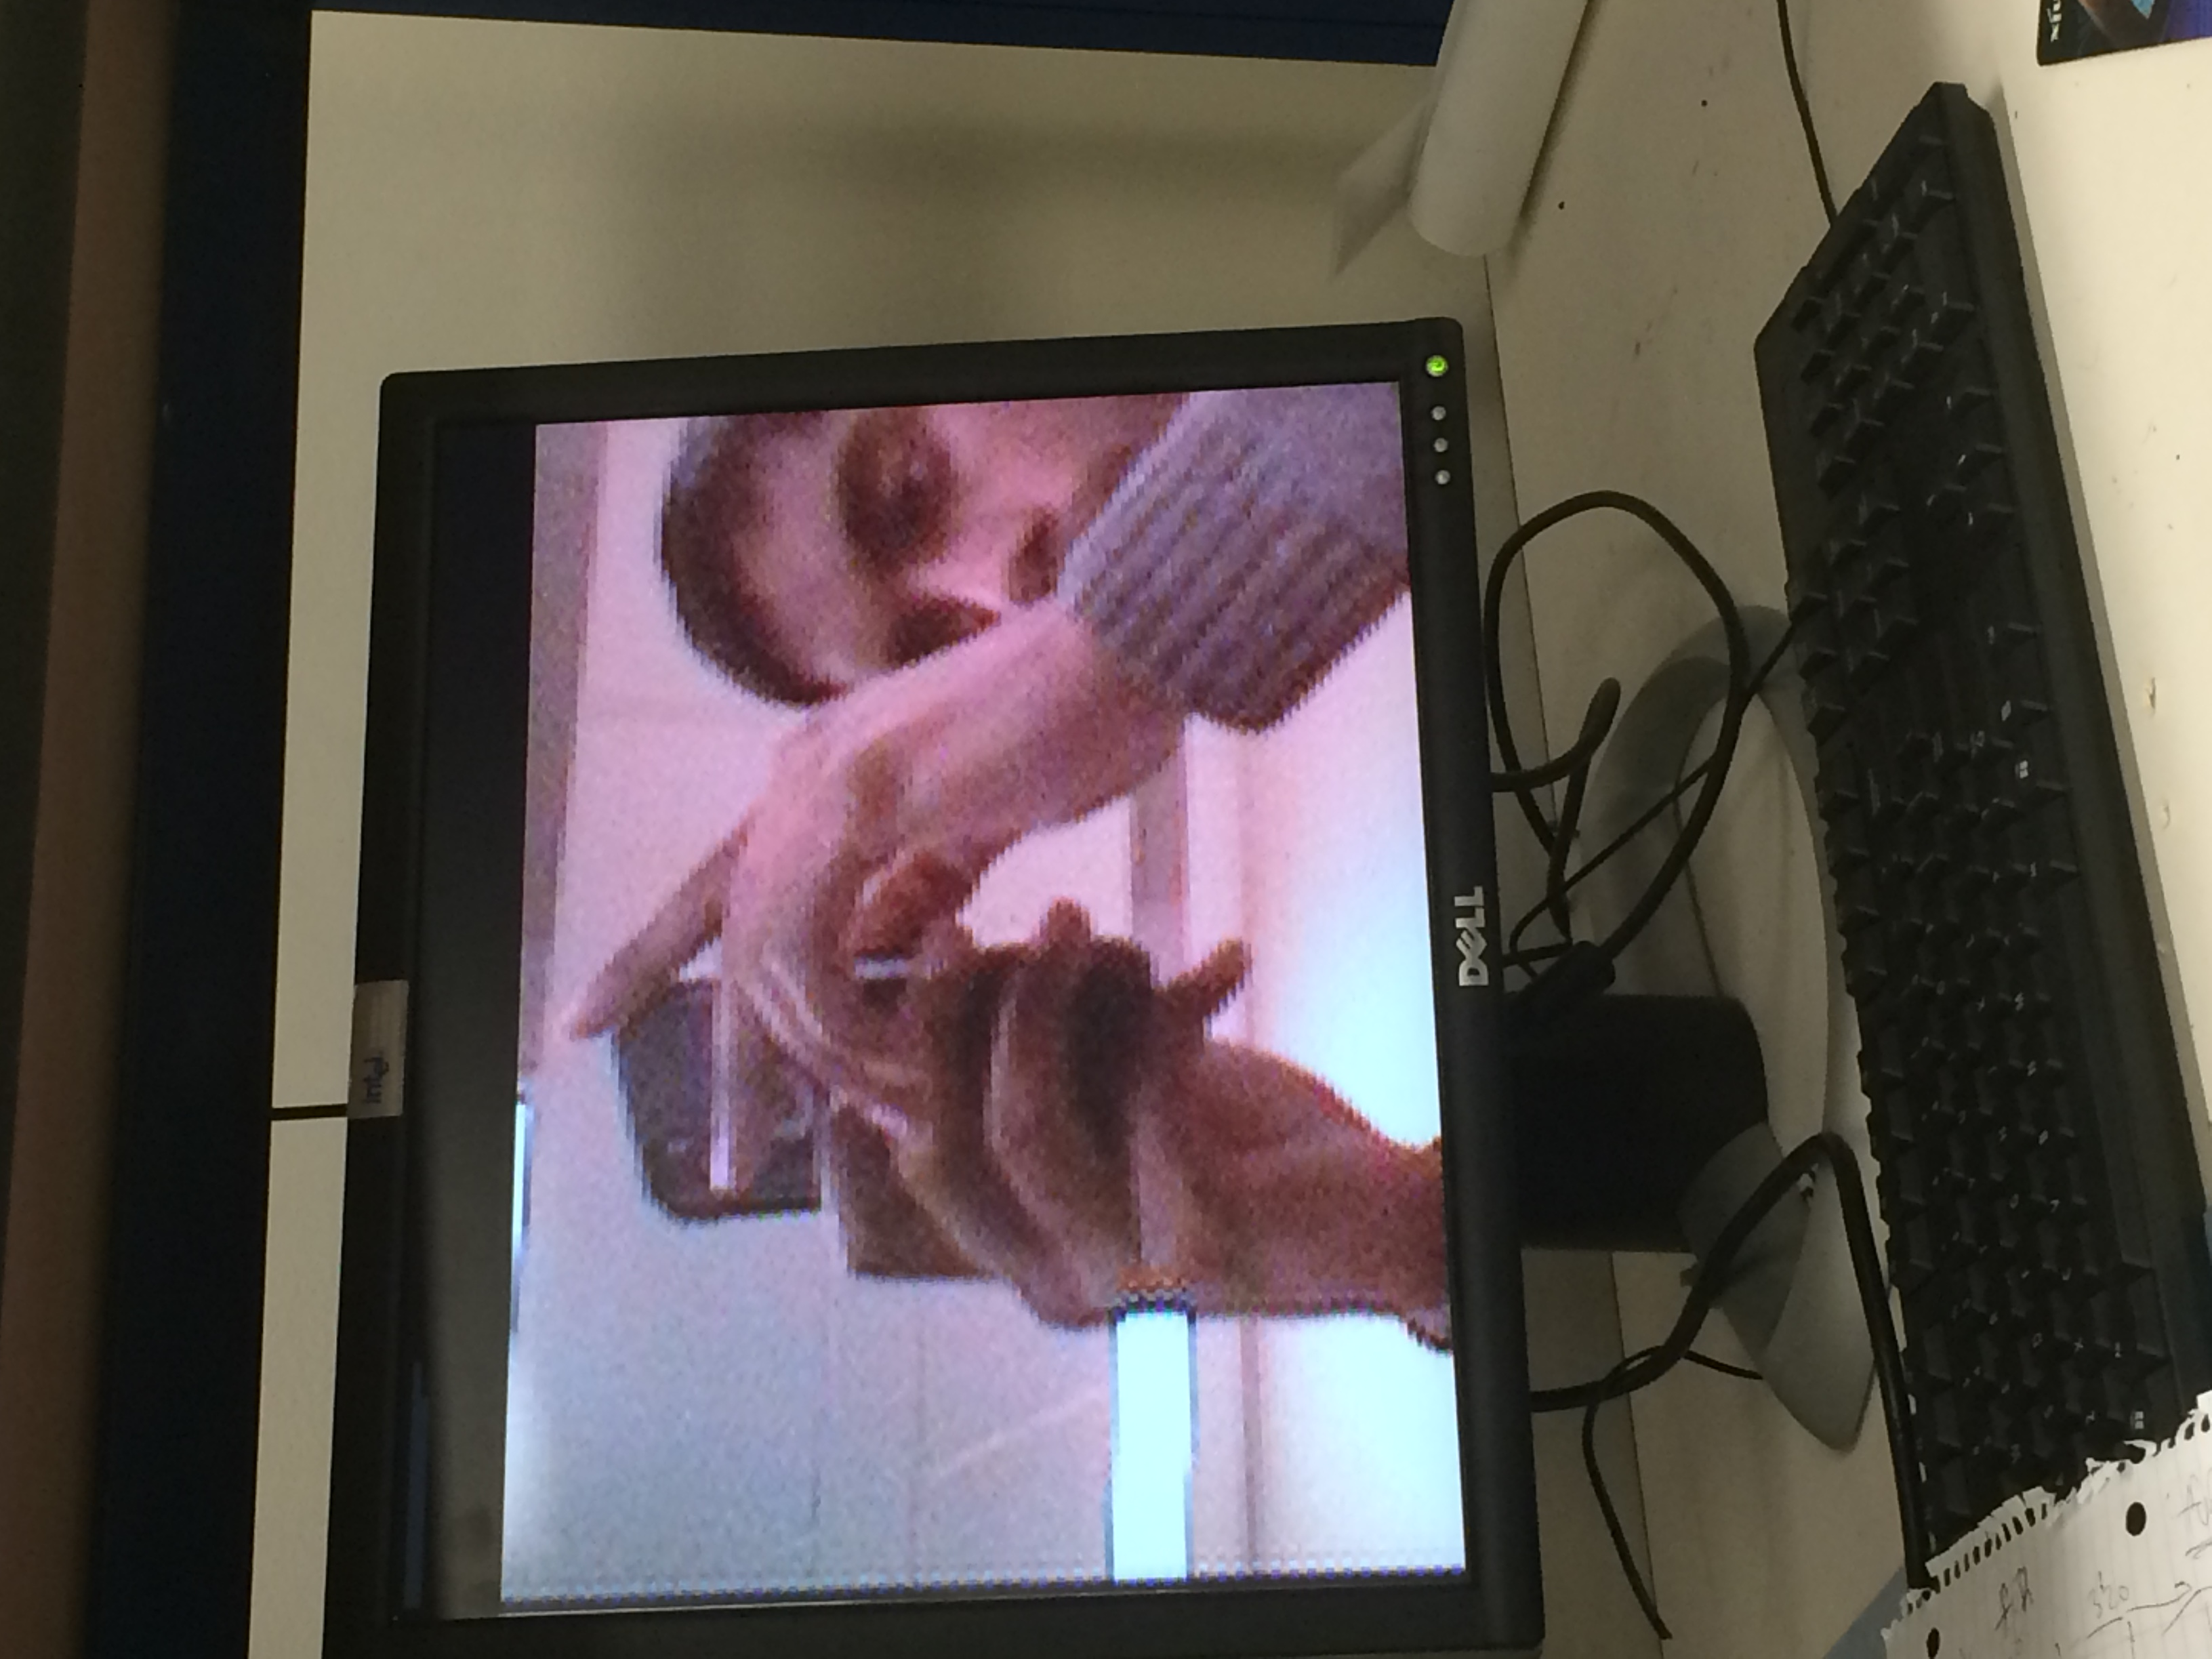
\includegraphics[width=0.8\textwidth, angle=270]{./img/ntsc-complete}
\end{figure}
\end{center}

TODO: ALL, COMPLETE WITH RESPECTIVE MODULES IN GORY DETAIL
ADD PICTURES WHEREVER APPROPRIATE
DO NOT ADD STAFF MODULES SEPARATELY, BUT DESCRIBE THEM IN OUR RELEVANT MODULES

\section{Final Product and User Interface}
Below is an image of our working system automatically correcting the input to a tilted projector so that it appears rectangular:
\begin{center}
\begin{figure}[H]
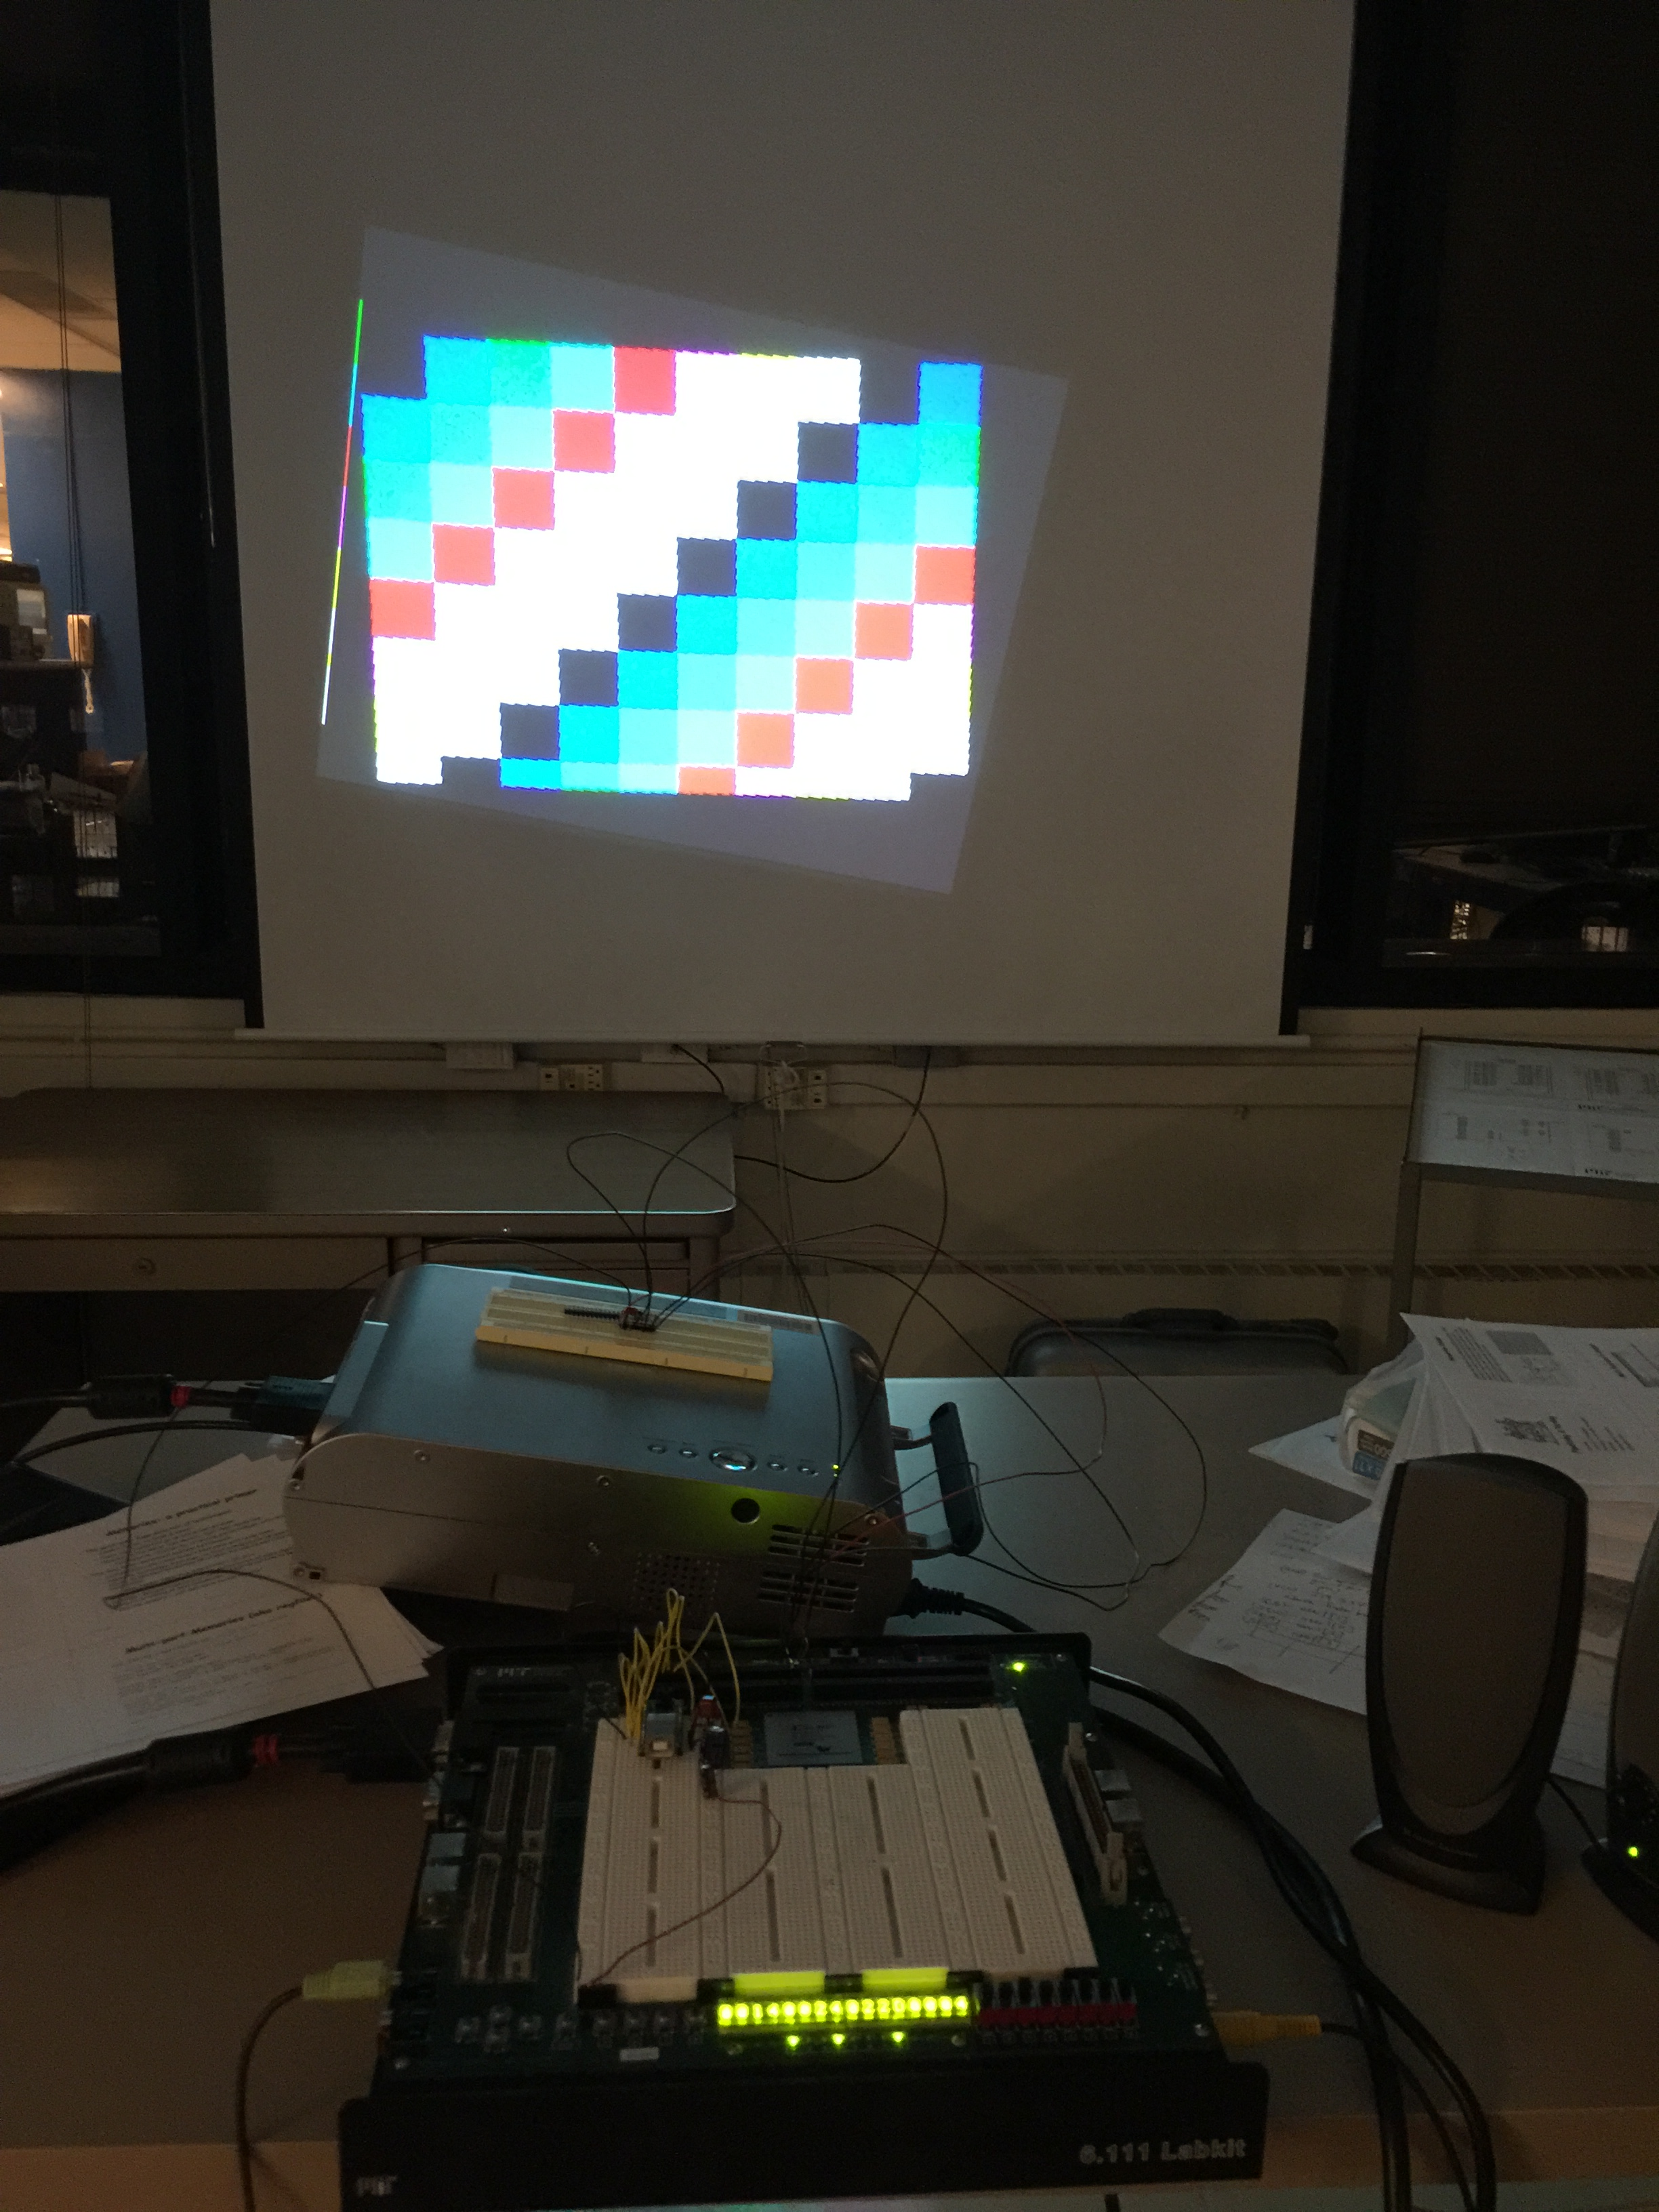
\includegraphics[width=0.8\textwidth]{./img/full-system}
\end{figure}
\end{center}
Below is an image of the user interface (UI) to our correction system:
\begin{center}
\begin{figure}[H]
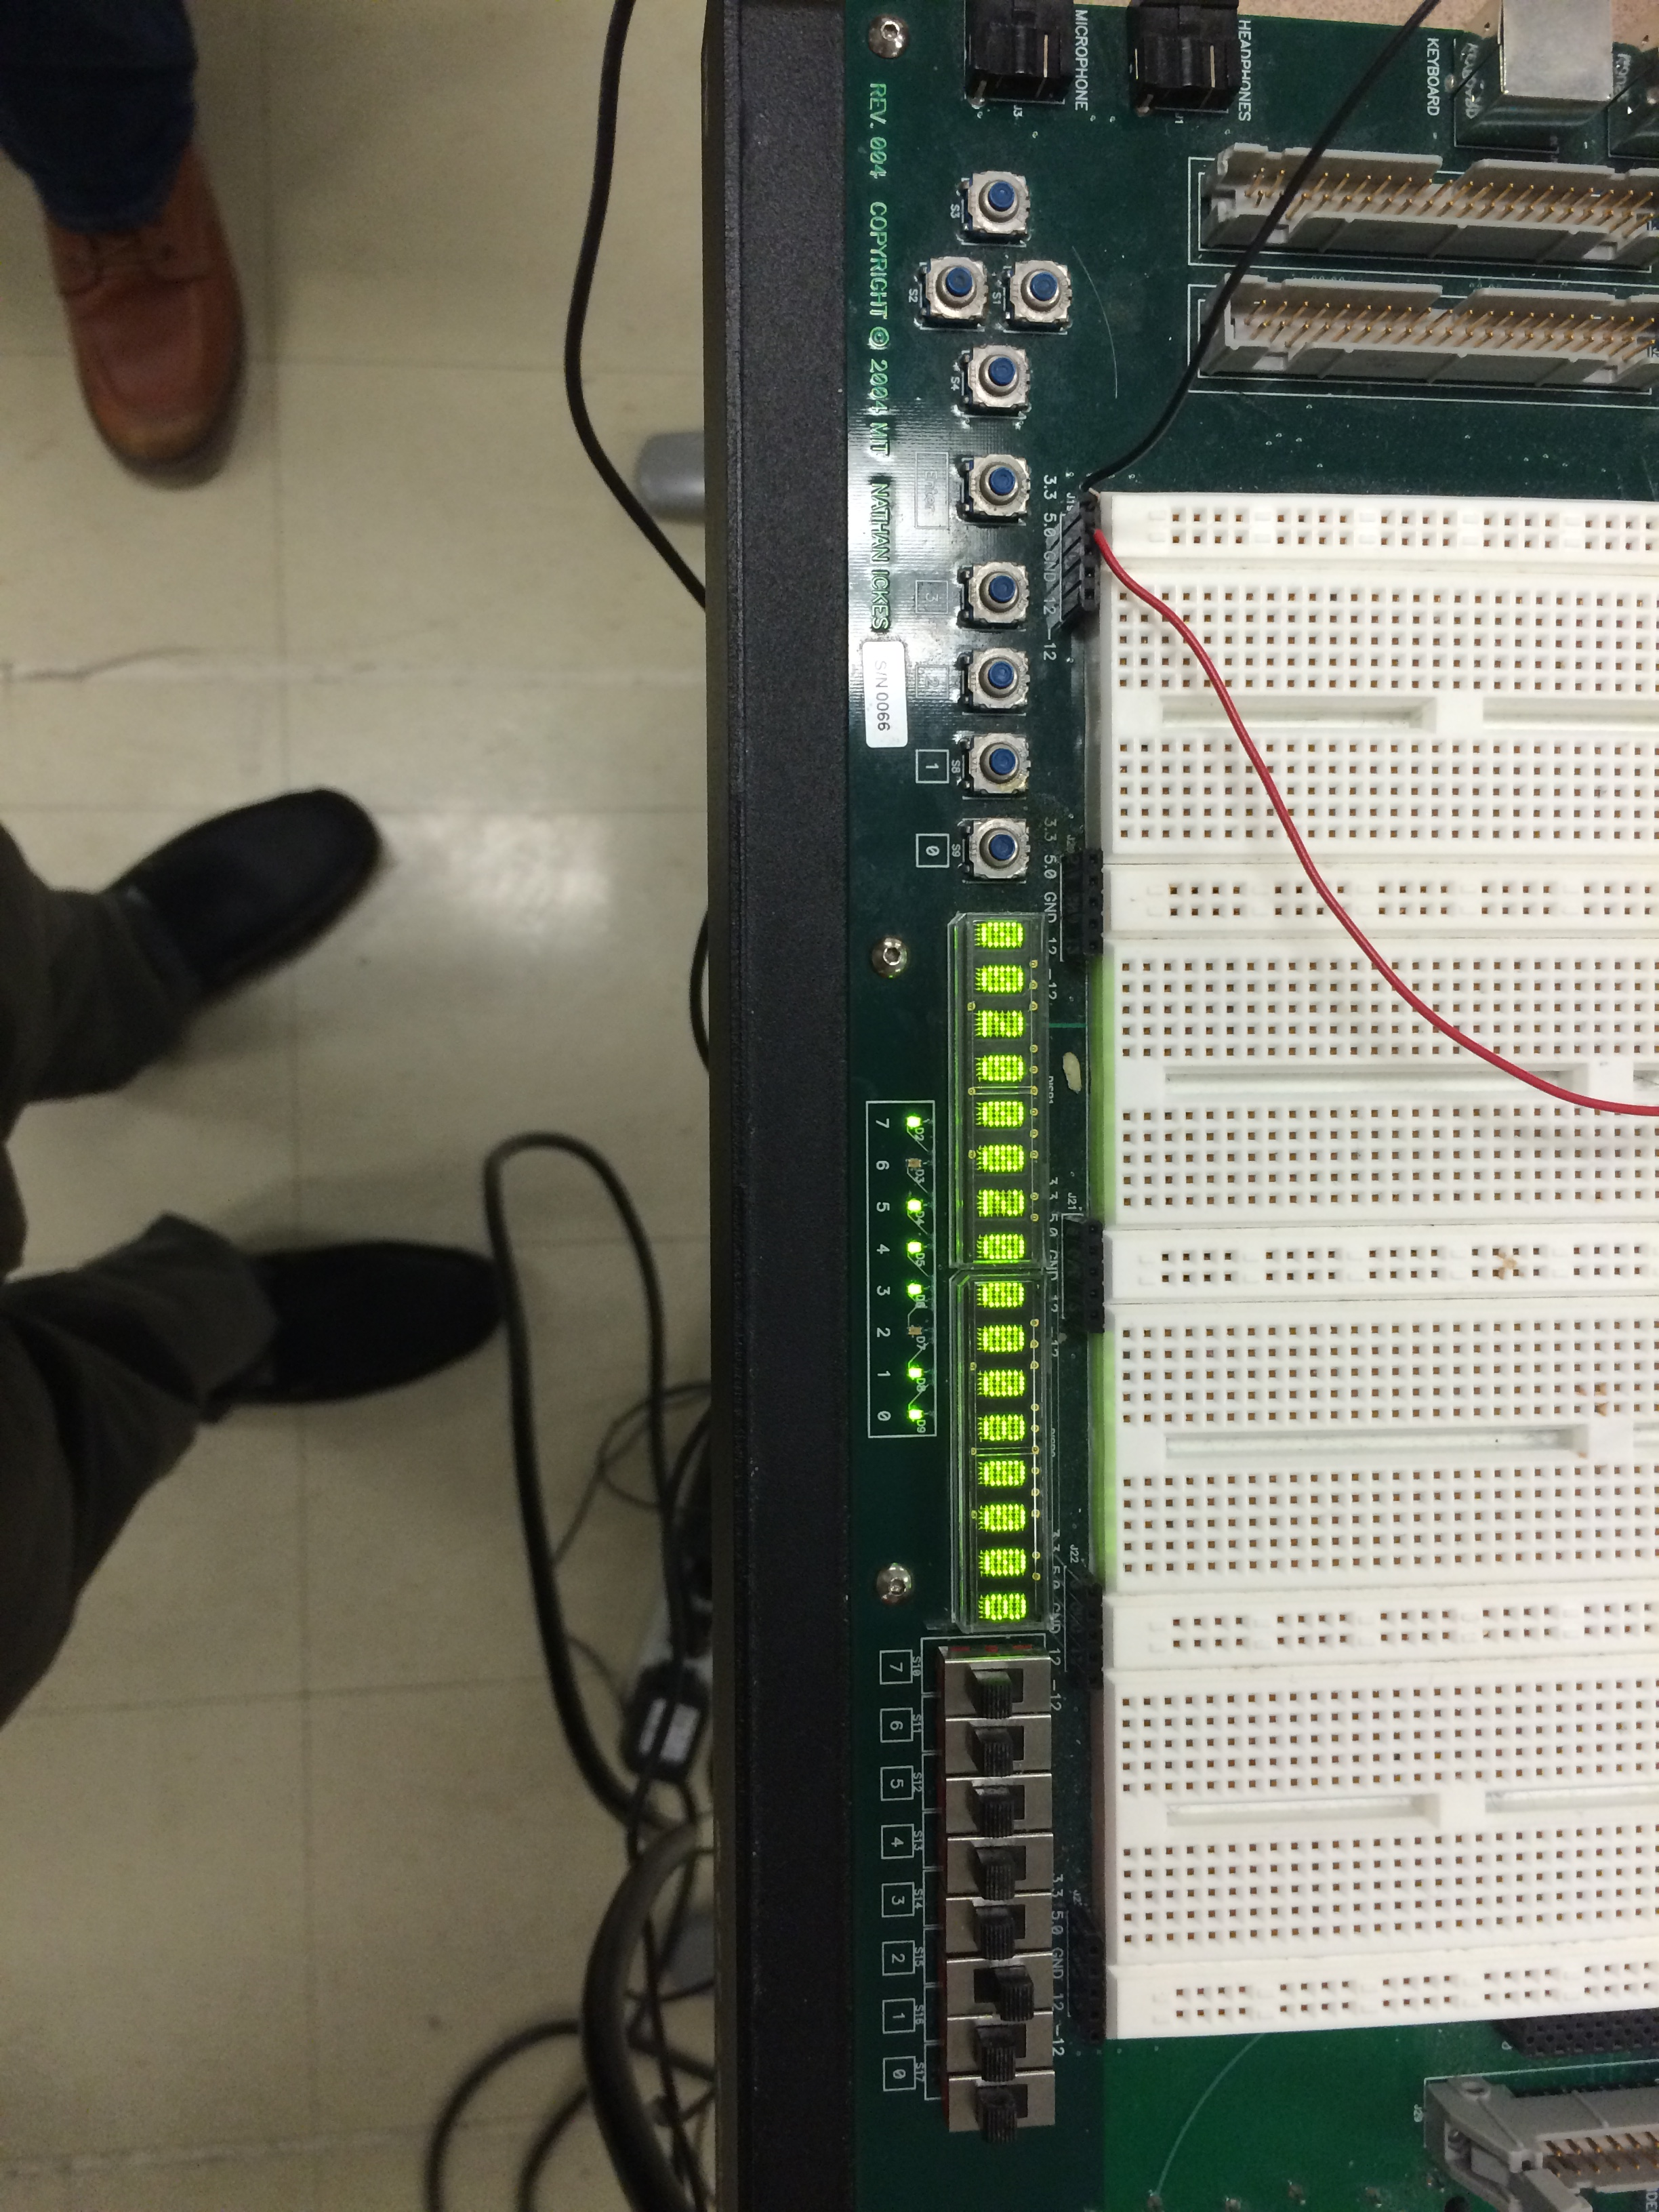
\includegraphics[width=0.8\textwidth, angle=90]{./img/ui}
\end{figure}
\end{center}
When pressed, button 0 triggers the audio system, which announces the percentage of screen pixels currently used for the corrected image. Buttons 2 and 3 adjust the volume of the audio system up or down. The first four digits on the hex display show the current x acceleration value, the next four show the current y acceleration value, the next four show the x coordinate of the corner of the quadrilateral selected by switches 0 and 1, and the last four show the y coordinate of this corner. If switch 7 is high, we are in manual correction mode, and the accelerometer readings are ignored and we can manually adjust the corner of the quadrilateral selected by switches 0 and 1 by pressing the up and down buttons (to adjust the x coordinate) and the left and right buttons (to adjust the y coordinate). When switch 5 is high, we display a checkerboard on the screen instead of the NTSC camera input.

\section{Testing And Debugging}

Testing and debugging Verilog-defined hardware is complicated due to the large synthesis times.
Unlike software, where one can change a single line of code,
and trigger an incremental build that can complete on the order of seconds,
synthesis of FGPA hardware is a lengthy process,
taking on the order of minutes or even hours depending on the amount of logic.
Our complete avoidance of Coregen modules definitely served us well in this respect.
We also consciously often commented out unnecessary modules.
This provided dual benefits:
\begin{itemize}
\item Much shorter synthesis times
\item Ensuring that the bug is being isolated as much as possible.
\end{itemize}
Nevertheless, these two steps are certainly not sufficient in efficient debugging.
As such, we adopted a multi-pronged testing and debugging approach.
Broadly speaking, we used the following methods:
\begin{itemize}
\item Icarus Verilog test benches/verification
\item Xilinx ModelSim test benches/verification
\item Julia implementations/tests of algorithms
\item Labkit I/O, e.g led's, hex display, logic analyzer probes
\item Staring at code/datasheets
\item Integration tests
\end{itemize}

\subsection{Icarus Verilog test benches/verification}
By far the most effective and efficient way of testing simple modules in our experience was the use of Icarus Verilog.
We are extremely grateful to a fellow student Andres for posting a note on our online discussion forum (Piazza) regarding the benefits and use of Icarus Verilog.
Defining and using test benches through Icarus Verilog is extremely easy and efficient.
In our experience, this was most useful for verifying long and complicated chains of combinational logic, such as mathematical algorithms.
It was also very useful for checking the syntax of our Verilog code.
As an example of its utility, we found a bug with perspective\_params that originated from incorrect mixed use of signed and unsigned arithmetic.
The main drawbacks of Icarus Verilog are its lack of visualizations of waveforms when invoked on the command line,
and its decreasing utility with complex state machines and other sequential logic.
The first of these drawbacks is addressed quite well by Xilinx ModelSim.

\subsection{Xilinx ModelSim test benches/verification}
ModelSim helped us to discover a bug in the staff-provided divider module. We instantiated a 79-bit divider and were not getting correct results. When we examined waveforms in ModelSim, we saw that the ready bit was being asserted far fewer than 79 cycles after we started the division. Upon closer examination of the module, it turned out that the counter the module was using to keep track of the current bit was only 6 bits wide, which supports only operand bit widths up to 63. We extended the width of this counter to 7 bits to solve this issue.

TODO: SHAWN describe any further work you did with ModelSim, especially something involving waveforms 

\subsection{Julia implementations/tests of algorithms}
Prior to implementing the perspective transforms on the FPGA,
we definitely wanted to verify the soundness of our approach in software first.
We settled on the use of the Julia programming language for this purpose,
though in all likelihood MATLAB or Python(+numpy/scipy/matplotlib) would have served just as well.
This was by far the most effective means of testing whether an algorithm is correct or not,
since one can rely on the benefits of fast debug/iterate cycles in software.
This is particularly true in the case of languages featuring a REPL (read, evaluate, print loop) based interpreter, such as Julia.
Correcting code is as simple as making some changes, reincluding the file in the REPL, and rerunning.
This helped us particularly in the verification of the pixels\_kept and perspective\_params module.
As an aside, to avoid using too many languages for software implementations,
we used Julia for our code generator for the accel\_lut as well.
As a concrete example of a serious bug caught using the help of our software implementations,
we were able to track and correct an error in the computation of $p_1$ and $p_2$ using this method.
Essentially, the bug was an interchange of two terms in the closed form expressions that occurred
while transcribing the closed form solutions we found for $p_1$ and $p_2$ from paper to the computer code.

\subsection{Labkit I/O}
We wired up the logic analyzer to the accelerometer pins to verify that the acc module was correctly initializing the accelerometer (e.g. the par\_to\_ser module was producing the correct serial bit stream for the register address and data). It turned out that the bug in the accelerometer was elsewhere (see the next section).

\subsection{Starting at code/datasheets}
This is definitely a questionable inclusion, and we do not recommend this method in general.
Nevertheless, it is often effective when done correctly and in the right spirit,
since it forces one to rethink and step through the logic again, questioning all assumptions.
For instance, once we confirmed that the divider implementation was incorrect,
we had to examine the divider code line by line.
It did not take us too long to realize the mistake in the implementation,
and looking back we do not see any other way of correcting the mistake.

As described in the section on the acc module, taking a second pass through the datasheet for the accelerometer helped us to identify an issue with a violated timing constraint ($t_{CS,DIS}$).
TODO: SHAWN, ADD ANY FURTHER INFO ON USE OF DATASHEETS
SHAWN - COMPACT FLASH/AUDIO DATASHEET

\subsection{Integration tests}
In addition to testing modules in isolation, we obviously also needed to test whether the modules work together or not.
Fortunately, the audio system could be quite easily separated from the rest of the system, so we anticipated easy integration here.
Ironically, we faced a strange problem here, which we never understood.
The issue was with the percentage value computed by pixels\_kept.
Initially, pixels\_kept was actually named pixels\_lost, and was computing 100 minus the percentage of pixels\_kept.
The audio module was written for percentage of pixels kept however,
so initially the audio module did a second subtraction from 100 to get the correct value.
The playback of the percentage was often incorrect for some reason (never identified).
Initially, we were keen on fixing the issue from the audio end, since pixels\_lost was a known correct module.
However, we had no luck fixing it from the audio end, so instead we renamed pixels\_lost to pixels\_kept and removed the subtraction from 100.
This somehow fixed the issue.

Much easier was the integration with the accelerometer.
This went flawlessly after we agreed upon the clock frequencies used by the accelerometer and the system. We made sure that the clocks used by the accelerometer and the accel\_lut (to which the accelerometer readings are sent) were integer multiples of one another to prevent any setup or hold time violations when clocks were out of phase.

Integration of the transformation logic with the memory interface was also extremely smooth,
apart from the subtle bug in address computation uncovered by our TA Jos\'{e}.

One of the most tedious aspects was the collection of data values for the lookup table.
It took around 2 hours of fiddling with the manual correction to get 12 readings for doing the interpolation.
The reason for this is that without appropriate measurement equipment,
it is hard to verify that the vertical edges of the checkerboard are exactly parallel to the vertical edges of the screen.
Furthermore, we also needed to ensure that the 4:3 aspect ratio was not distorted.

\section{Future Work}
Although our projector tilt compensation system met most of our initial goals,
there are a wide variety of extensions and modifications to the project that we would have liked to implement.

On the image side, we would like to take some steps to improve the quality of the projected image.
As noted earlier, one of our key design decisions was the use of reduced resolution ($320 \times 240$) and reduced color depth (12 bit as opposed to 24 bit).
This can be achieved with either a labkit with more dual-ported memory, or our existing labkit with a sophisticated ZBT based memory design (with an arbiter).
Another improvement that can be made to the images is the use of some sort of anti-aliasing filter.
For instance, when we compute the coordinates in the pixel\_map module, we only look at the integer part of the division (corresponding to a single pixel index).
By looking at the fractional part, we could interpolate the color values at neighboring pixels and use that to reduce the ``jagged edges'' associated with aliasing in images.

Another big unknown is how well the accelerometer approach works when the projector is not kept at a fixed distance from the screen.
We have not tested whether this would affect the quality of the automatic correction.
If this does affect quality, we are confident that by adding an additional distance sensor,
we could simply incorporate the distance values into the lookup table and make the automatic correction usable again.
Of course, the lookup table could become very large if we do this.
There are two avenues around this:
\begin{itemize}
    \item Store the lookup table in a larger memory, e.g ZBT.
    \item A more scalable approach is to start doing interpolation in the hardware itself.
        This will require additional hardware resources and more logic,
        but the size of the logic will only grow with the number of data points,
        as opposed to the number of bits coming from the sensors.
\end{itemize}

On the audio side as well, there are many avenues for substantial improvement.
TODO: SHAWN - TALK ABOUT AUDIO FUTURE WORK, TIE IT IN WITH YOUR CURRENT ISSUES

Another useful feature which we unfortunately did not have time to implement is persistent storage of a user's manual correction settings.
After all, no matter how good the accel\_lut is, it is extremely likely that with certain extreme orientations,
the settings obtained through the lookup table are unsatisfactory.
One option for dealing with this would be saving manual override settings into some non-volatile storage such as flash,
and using them on the next power cycle.
Given our issues with compact flash in the audio domain, progress on this front would likely be negligible.
Hopefully, with an improved labkit, we would not run into the flash issues.

\section{Conclusion}
Our projector tilt compensation system used digital logic to successfully perform a perspective transform on an image.
This enables fully general manual correction of distortions of the projected image on the screen.
Moreover, we also created an automatic correction system for correction of distortion resulting from 2 axes of tilt
via the usage of an accelerometer that would sense the angle of tilt along these two axes.
We also implemented a useful audio features regarding the percentage of pixels kept by our correction system.

We believe that there were a number of factors that allowed us to succeed with this project.
First and foremost, we started early and tackled potential issues as early as possible, with a consistent time commitment every week.
Second, we spent a lot of time doing software simulations/verifications before diving in and writing Verilog.
The rationale behind this is that correction and testing in software is much faster than synthesis on the FPGA.
Third, we had regular meetings among ourselves to ensure that issues some member of our team had would be addressed collectively.

Overall, we are satisfied with the quality of this system,
especially considering the time limitations/scope of this project.
We are confident that with some additional work,
this system could truly rival commercial offerings in this space.

\bibliographystyle{plainnat}
\bibliography{references}
\newpage

\appendix

\section{Source Code}
Source code for the project may be obtained on GitHub: \url{https://github.com/gajjanag/6111_Project}.
For completeness, we include all source code here as well.
For ease of browsing through the code, we have divided the modules into roughly three categories:
\begin{itemize}
\item Staff Modules: modules that are essentially the same as staff provided modules, with minor modifications for our specific needs.
\item Labkit: top level labkit module with general instantiations, including clock generators, and ucf file
\item Our Modules: modules created by us for our project
\end{itemize}

% For fast compilation, disable inclusion of source code files
% Include these for final submission
%\begin{comment}
\subsection{Staff Modules}
\subsubsection{debounce.v}
\inputminted[linenos]{verilog}{../../src/debounce.v}
\subsubsection{delay.v}
\inputminted[linenos]{verilog}{../../src/delay.v}
\subsubsection{display\_16hex.v}
\inputminted[linenos]{verilog}{../../src/display_16hex.v}
\subsubsection{vga.v}
\inputminted[linenos]{verilog}{../../src/vga.v}
\subsubsection{divider.v}
\inputminted[linenos]{verilog}{../../src/divider.v}
\subsubsection{ycrcb2rgb.v}
\inputminted[linenos]{verilog}{../../src/ycrcb2rgb.v}
\subsubsection{ntsc2zbt.v}
\inputminted[linenos]{verilog}{../../src/ntsc2zbt.v}
\subsubsection{video\_decoder.v}
\inputminted[linenos]{verilog}{../../src/video_decoder.v}
\subsubsection{flash\_int.v}
\inputminted[linenos]{verilog}{../../assets/flash_IO/flash_int.v}
\subsubsection{flash\_manager.v}
\inputminted[linenos]{verilog}{../../assets/flash_IO/flash_manager.v}
\subsubsection{test\_fsm.v}
\inputminted[linenos]{verilog}{../../assets/flash_IO/test_fsm.v}
\subsubsection{usb\_input.v}
\inputminted[linenos]{verilog}{../../assets/USB_Transfer/usb_input.v}
\subsubsection{usb\_transfer\_script.py}
\inputminted[linenos]{python}{../../assets/usb_transfer_script.py}


\subsection{Labkit}
\subsubsection{labkit.v}
\inputminted[linenos]{verilog}{../../src/labkit.v}
\subsubsection{labkit.ucf}
\inputminted[linenos]{verilog}{../../src/labkit.ucf}

\subsection{Our Modules}
\subsubsection{acc.v}
\inputminted[linenos]{verilog}{../../src/acc.v}
\subsubsection{accel\_lut.v}
\inputminted[linenos]{verilog}{../../src/accel_lut.v}
\subsubsection{accel\_lut.jl}
\inputminted[linenos]{julia}{../../src/accel_lut.jl}
\subsubsection{accel\_lut.txt}
\inputminted[linenos]{todotxt}{../../src/accel_lut.txt}
\subsubsection{pixels\_kept.v}
\inputminted[linenos]{verilog}{../../src/pixels_kept.v}
\subsubsection{bram.v}
\inputminted[linenos]{verilog}{../../src/bram.v}
\subsubsection{addr\_map.v}
\inputminted[linenos]{verilog}{../../src/addr_map.v}
\subsubsection{slow\_clk.v}
\inputminted[linenos]{verilog}{../../src/slow_clk.v}
\subsubsection{move\_cursor.v}
\inputminted[linenos]{verilog}{../../src/move_cursor.v}
\subsubsection{perspective\_params.v}
\inputminted[linenos]{verilog}{../../src/perspective_params.v}
\subsubsection{pixel\_map.v}
\inputminted[linenos]{verilog}{../../src/pixel_map.v}
\subsubsection{audioManager.v}
\inputminted[linenos]{verilog}{../../src/audioManager.v}
\subsubsection{binaryToDecimal.py}
\inputminted[linenos]{python}{../../assets/binaryToDecimal.py}
\subsubsection{BCD.v}
\inputminted[linenos]{verilog}{../../src/BCD.v}
\subsubsection{ClockDivider.v}
\inputminted[linenos]{verilog}{../../src/ClockDivider.v}
\subsubsection{Square.v}
\inputminted[linenos]{verilog}{../../src/Square.v}
%\end{comment}

\end{document}
